\makeatletter
\def\input@path{{../}}
\makeatother
\documentclass[../master_thesis.tex]{subfiles}
\begin{document}
\chapter{Results}\label{chap:Results}
\section{Overview of tests}
We divided the tests of this implementation into four main types, (1) theoretical
correctness, (2) parametrization, (3) comparison and (4) tests of the variational implementation.
\begin{enumerate}

\item \textbf{Theoretical correctness:}
In the tests of theoretical correctness we test if our implementation gives the
results to problems as expected. The tests for this were comparisons to
the energy of  \ce{Li^+} in an environment with dielectric constant $\epsinf$
with the value we would get from the Born model. In the Born model the energy of a  %citation please
one-atom ion in a solvent is the same as the energy of a point charge in the same solvent.
This energy is described as \cite{Tomasi:1994wt}
\begin{equation}\label{eq:bornenergy}
  E_{R}^{Born} =-\frac{\epsilon-1}{2 \epsilon} \frac{q^{2}}{R}
\end{equation}
In the Born model the cavity is defined as a sharp two-dimensional surface. Because of this
it is not expected that our results, with a smooth cavity, should converge to the same values as
the Born model.
A second comparison was done with Gauss' theorem\cite{Sorland} where we tested for the
following relation that should hold for a point charge
\begin{equation}\label{eq:Reactioncharge}
  \int \gamma_s \text{d}r= \frac{1 - \epsinf }{\epsinf} q
\end{equation}
the integral evaluates the reaction charge of the system.

\item \textbf{Parametrization:} The parametrization tests were done by changing one parameter at a time while
comparing this same change to Gaussian calculations with different basis sets.
First we only checked the dependency on the radius and how changing it would
affect the reaction field energy with respect to Gaussian calculations of the same
radii. We then compared Gaussian calculations of radius $R$ against \mrchem
calculations of radius $R+0.2$ in an attempt to see an improvement in the
results.
A second parametrization test was done with only \ce{Li^+}
where we changed the relative precision of the \mrchem calculations to see how
they affect the energy with respect to the Gaussian energies. This was also done
on different radii.

\item \textbf{Comparison:} We then took 4 molecules that were tested by Chipman in \cite{Chipman2002} and compared the
results from the computations against Gaussian results. The molecules used
were \ce{H_2O}, \ce{NO^+}, \ce{CN^-} and \ce{CH_3CONH_2}. These tests are classified into
spherical cavity tests and molecular-shaped cavity tests. Spherical cavity tests are performed
by varying the radius of the cavities for each molecule. The spherical cavity test was done for
all molecules except for \ce{CH_3CONH_2} as it was too big, which made calculations
in both Gaussian and \mrchem extremely slow.

The molecular-shaped cavity tests consist of making interlocking spheres centered on
each atom with radius equal to the atom's van der Waals radius. The set of radii by
 Bondi \cite{doi:10.1021/j100785a001} are scaled by $1.2$ as outlined by \cite{Tomasi:1994wt}.
 These radii were later shifted by $0.2$ Bohr so that we were comparing
 \mrchem calculations of bigger radii to Gaussian calculations.

\item \textbf{Variational tests:} As stated before in Chapters \ref{chap:Solvent_effect} and \ref{chap:implementation}
a variational formulation of the reaction field Problem was implemented in this thesis,
The tables in Appendix \ref{Datatables} show a row which is labeled "Variational",
though the variational implementation behaved in a irregular way. We will show
the reaction energy plots for the variational implementation for both \ce{H_2O}
and \ce{Li^+} as those are the ones that had the most data points. We leave the
reader to evaluate the variational energies for the other molecules.

\end{enumerate}
All \mrchem tests were done with relative precision of $1e-6$, RHF method and \verb!SAD_DZ! as a
starting guess \cite{MRchem}. All Gaussian calculations were ran with \ac{HF} method,  Dunning's correlation
consistent basis sets\cite{doi:10.1063/1.456153} of increasing completeness, \verb!scrf(pcm, read)! option with
\verb!nocav!, \verb!nodis! and  \verb!norep! keywords. Both Gaussian and \mrchem computations were run with
optimized geometries from Gaussian using \verb!b3lyp/cc-pVQZ!.

\section{Data}
\subsection{Theoretical correctness tests}
We calculated the integral on the left hand side of Equation \ref{eq:Reactioncharge} for a point charge
with charge $q=3$ and compared it to the exact value calculated as shown in the right hand side of the same
equation. This is shown in Tables \ref{tab:Intgamma2} and \ref{tab:intgamma80}.

We then evaluated the reaction field energy of the same point charge and compared it
to an exact value calculated as in Equation  \ref{eq:bornenergy}. Tables \ref{tab:Er2}
and \ref{tab:Er80} show this.

For both the tests above we calculated the values with two radii, $R = 3.0,\ 4.0$ Bohr,
two sets of dielectric constants, $\epsinf = 2,\ 80$, two transition widths, $\sigma = 0.1,\ 0.2$,
and two values for the relative precision, $1e-4,\ 1e-6$.

\begin{table}[!htbp]
\caption[Reaction charge for $\epsinf = 2$]{Reaction charge for a point charge of $q = 3$ and $\epsinf = 2$ calculated with differing precision, transition width ($\sigma$) and cavity radius (Bohr) compared to the exact values}
\resizebox{\textwidth}{!}{
\begin{tabular}{l|r|r|r|r|r}

Radius & \multicolumn{1}{l|}{Prec.} & $\sigma = $0.2 & \multicolumn{1}{l|}{Rel. Diff.} & $\sigma = $0.1 & \multicolumn{1}{l|}{Rel. Diff.} \\ \hline
\multicolumn{ 1}{r|}{3.0} & 1E-04 & -1.499964 & -2.41E-05 & -1.504559 & 3.04E-03 \\
\multicolumn{ 1}{l|}{} & 1E-06 & -1.499999 & -7.43E-07 & -1.500001 & 4.17E-07 \\ \hline
\multicolumn{ 1}{r|}{4.0} & 1E-04 & -1.499602 & -2.66E-04 & -1.503913 & 2.61E-03 \\
\multicolumn{ 1}{l|}{} & 1E-06 & -1.500002 & 1.21E-06 & -1.499659 & -2.27E-04 \\ \hline
\multicolumn{ 1}{|l|}{Exact} & \multicolumn{1}{|l|}{} & -1.500000 & \multicolumn{1}{l|}{} & -1.500000 & \multicolumn{1}{l|}{} \\ \hline
\end{tabular}}
\label{tab:Intgamma2}
\end{table}

\begin{table}[!htbp]
  \caption[Reaction charge for $\epsinf = 80$]{Reaction charge for a point charge of $q = 3$ and $\epsinf = 80$ calculated with differing precision, transition width ($\sigma$) and cavity radius (Bohr) compared to the exact values}
  \resizebox{\textwidth}{!}{
  \begin{tabular}{l|r|r|r|r|r}
    Radius & \multicolumn{1}{l|}{Prec.} & $\sigma = $0.2 & \multicolumn{1}{l|}{Rel. Diff.} & $\sigma = $0.1 & \multicolumn{1}{l}{Rel. Diff.} \\ \hline
    \multicolumn{ 1}{r|}{3.0} & 1.00E-04 & -2.96495 & 8.26E-04 & -2.96167 & -2.81E-04 \\
    \multicolumn{ 1}{l|}{} & 1.00E-06 & -2.96250 & 2.92E-07 & -2.96235 & -5.16E-05 \\ \hline
    \multicolumn{ 1}{r|}{4.0} & 1.00E-04 & -2.96400 & 5.06E-04 & -2.95605 & -2.18E-03 \\
    \multicolumn{ 1}{l|}{} & 1.00E-06 & -2.96243 & -2.20E-05 & -2.96215 & -1.17E-04 \\ \hline
    \multicolumn{ 1}{|l|}{Exact} & \multicolumn{1}{|l|}{} & -2.96250 & \multicolumn{1}{l|}{} & -2.96250 & \multicolumn{1}{l|}{} \\ \hline
  \end{tabular}}
  \label{tab:intgamma80}
\end{table}

\begin{table}[!htbp]
\caption[Reaction field energy for a point charge of $\epsinf = 2$]{Reaction field energy for a point charge of $q = 3$ and $\epsinf = 2$ calculated with differing precision, transition width ($\sigma$) and cavity radius (Bohr) compared to the values from the Born model}
\resizebox{\textwidth}{!}{
\begin{tabular}{l|l|r|r|r|r|r}
Radius & Born energy & \multicolumn{1}{l|}{Prec.} & $\sigma = $0.2 & \multicolumn{1}{l|}{Rel. Diff.} & $\sigma = $0.1 & \multicolumn{1}{l|}{Rel. Diff.} \\ \hline
\multicolumn{1}{r|}{3.0} & \multicolumn{ 1}{r|}{-0.7500} & \multicolumn{ 1}{r|}{1E-04} & -0.7586 & 1.14E-02 & -0.7560 & 7.96E-03 \\
 & \multicolumn{ 1}{l|}{} & \multicolumn{ 1}{r|}{1E-06} & -0.7586 & 1.15E-02 & -0.7539 & 5.15E-03 \\ \hline
\multicolumn{1}{r|}{4.0} & \multicolumn{ 1}{r|}{-0.5625} & \multicolumn{ 1}{r|}{1E-04} & -0.5670 & 7.95E-03 & -0.5660 & 6.27E-03 \\
 & \multicolumn{ 1}{|l|}{} & \multicolumn{ 1}{r|}{1E-06} & -0.5671 & 8.17E-03 & -0.5645 & 3.53E-03 \\
\end{tabular}}
\label{tab:Er2}
\end{table}

\begin{table}[!htbp]
\caption[Reaction field energy for a point charge of $\epsinf = 80$]{Reaction field energy for a point charge of $q = 3$ and $\epsinf = 80$ calculated with differing precision, transition width ($\sigma$) and cavity radius (Bohr) compared to the values from the Born model}
\resizebox{\textwidth}{!}{
\begin{tabular}{l|l|r|r|r|r|r}
Radius & Born energy & \multicolumn{1}{l|}{Prec.} & $\sigma = $0.2 & \multicolumn{1}{l|}{Rel. Diff.} & $\sigma = $0.1 & \multicolumn{1}{l|}{Rel. Diff.} \\ \hline
\multicolumn{1}{r|}{3} & \multicolumn{ 1}{r|}{-1.48125} & 1.00E-04 & -1.55781 & 5.17E-02 & -1.51700 & 2.41E-02 \\
 & \multicolumn{ 1}{l|}{} & 1.00E-06 & -1.55658 & 5.09E-02 & -1.51731 & 2.43E-02 \\ \hline
\multicolumn{1}{r|}{4} & \multicolumn{ 1}{r|}{-1.1109375} & 1.00E-04 & -1.15306 & 3.79E-02 & -1.12961 & 1.68E-02 \\
 & \multicolumn{ 1}{l|}{} & 1.00E-06 & -1.15241 & 3.73E-02 & -1.13093 & 1.80E-02 \\
\end{tabular}}
\label{tab:Er80}
\end{table}

\clearpage


\subsection{Parametrization Tests}\label{sec:paratests}
We first varied the radius of the cavity for \ce{H_2O} and lithium. The following
Table \ref{tab:rawwaterdata}  presents the data for the energy
calculations of \ce{H_2O} with the three first cavity radii used in the calculations
These are the total  energy of the system including the solvent effect contributions.
\begin{table}[!htbp]
  \caption[$E_{tot}$ for \ce{H_2O} in Water sample]{Total Energy Calculations example for \ce{H_2O} in Water. Energy in Hartree and radii of the cavity in Bohr}
  \begin{center}
    \begin{tabular}{l|r|r|r}
      Basis & $R =3.6$ & $R=3.7$ & $R=3.8$ \\  \hline
      cc-pVDZ & -7.6039e+01 & -7.6038e+01 & -7.6036e+01 \\
      cc-pVTZ & -7.6070e+01 & -7.6069e+01 & -7.6067e+01 \\
      cc-pVQZ & -7.6078e+01 & -7.6076e+01 & -7.6075e+01 \\
      cc-pV5Z & -7.6080e+01 & -7.6079e+01 & -7.6077e+01 \\\hline
      aug-cc-pVDZ & -7.6054e+01 & -7.6053e+01 & -7.6052e+01 \\
      aug-cc-pVTZ & -7.6074e+01 & -7.6072e+01 & -7.6071e+01 \\
      aug-cc-pVQZ & -7.6079e+01 & -7.6077e+01 & -7.6076e+01 \\
      aug-cc-pV5Z & -7.6080e+01 & -7.6079e+01 & -7.6077e+01 \\\hline
      daug-cc-pVDZ & -7.6055e+01 & -7.6053e+01 & -7.6052e+01 \\
      daug-cc-pVTZ & -7.6074e+01 & -7.6072e+01 & -7.6071e+01 \\
      daug-cc-pVQZ & -7.6079e+01 & -7.6077e+01 & -7.6076e+01 \\
      daug-cc-pV5Z & -7.6080e+01 & -7.6079e+01 & -7.6077e+01 \\\hline
      \mrchem & -7.6085E+01 & -7.6083E+01 & -7.6081E+01 \\
    \end{tabular}
  \end{center}
  \label{tab:rawwaterdata}
\end{table}

To calculate the reaction field energy we took a gas phase calculation
of a basis set and subtracted it from the total energy calculated with the same
basis set. In \mrchem this was done using the same relative precision for both
the gas phase and the solvent calculations. The following equation was used to
calculate the reaction field Energy $E_r$
\begin{equation}\label{eq:deltaer}
  E_r = E_{tot} - E_{vac}
\end{equation}
Examples of $E_r$ for the first three cavity radii for \ce{H_2O} obtained from the operation
in Equation \ref{eq:deltaer} can be seen in Table \ref{tab:Erwatdata}

\begin{table}[!htbp]
\caption[$E_r$ for \ce{H_2O} in Water sample]{Reaction Field Energy Calculations example for \ce{H_2O} in water, Energy in Hartree and radii of the cavity in Bohr}
\begin{center}
\begin{tabular}{l|r|r|r|r}
Basis & 3.6 & 3.7 & 3.8 \\\hline
cc-pVDZ & -1.2450E-02 & -1.0998E-02 & -9.7804E-03 \\
cc-pVTZ & -1.3097E-02 & -1.1545E-02 & -1.0243E-02 \\
cc-pVQZ & -1.3218E-02 & -1.1651E-02 & -1.0334E-02 \\
cc-pV5Z & -1.3284E-02 & -1.1713E-02 & -1.0393E-02 \\\hline
aug-cc-pVDZ & -1.3190E-02 & -1.1634E-02 & -1.0328E-02 \\
aug-cc-pVTZ & -1.3238E-02 & -1.1670E-02 & -1.0353E-02 \\
aug-cc-pVQZ & -1.3221E-02 & -1.1655E-02 & -1.0338E-02 \\
aug-cc-pV5Z & -1.3223E-02 & -1.1655E-02 & -1.0337E-02 \\\hline
daug-cc-pVDZ & -1.3228E-02 & -1.1665E-02 & -1.0351E-02 \\
daug-cc-pVTZ & -1.3243E-02 & -1.1675E-02 & -1.0357E-02 \\
daug-cc-pVQZ & -1.3223E-02 & -1.1656E-02 & -1.0340E-02 \\
daug-cc-pV5Z & -1.3224E-02 & -1.1655E-02 & -1.0337E-02 \\\hline
\mrchem & -1.8036E-02 & -1.5494E-02 & -1.3437E-02 \\
\end{tabular}
\end{center}
\label{tab:Erwatdata}
\end{table}
 The Tables \ref{tab:rawwaterdata} and \ref{tab:Erwatdata} do not show the total
 amount of results that were used to plot the Energies. The results for the remaining
 radii can be seen in Appendix \ref{Datatables}.

We now plot the data from the total energy and reaction energy tables for
both \ce{H_2O} and \ce{Li^+}. In this chapter we will be plotting only against
double augmented basis sets. The rest of the plots for the other basis sets can
be seen in Appendix \ref{Figures}.

The plots for the reaction energy of \ce{H_2O} for
both the Gaussian and  \mrchem calculations can be seen in Figure \ref{fig:watEnergyplotsdaug}.
The same type of plots for \ce{Li^+} can be seen in Figure \ref{fig:lipEnergyplotsdaug}.
In both of these figures we are comparing the energy from \mrchem to sets of four
curves formed each of double, triple, quadruple and quintuple zeta Dunning's correlation
consistent basis sets\cite{doi:10.1063/1.456153} as implemented in Gaussian \cite{G09}.

The \mrchem energy values $E_{MRChem}$ for each radius were compared to the
corresponding values of each of the different basis set calculations in
Gaussian  $E_{Gaussian}^{basis}$ by finding the relative difference $d_r$
between them as
\begin{equation}\label{eq:reldiff}
  d_r = \frac{E_{Gaussian}^{basis} - E_{MRChem}}{E_{MRChem}}
\end{equation}
The operation in Equation \ref{eq:reldiff} was applied to both \ce{H_2O} and \ce{Li^+}.
The results for \ce{H_2O} and \ce{Li^+} are presented in Figures \ref{fig:watreldiffdaug}
and \ref{fig:lipreldiffdaug} respectively.

We then shifted the cavity radius of the \mrchem calculations for both \ce{H_2O} and
\ce{Li^+} so they were $0.2$ Bohr bigger and compared them to Gaussian calculations
with an unshifted radius. The relative Difference plots for \ce{H_2O} and \ce{Li^+} can be seen
in Figures \ref{fig:watreldiff02daug} and \ref{fig:lipreldiff02daug} respectively.

Lastly we computed the reaction field energies of \ce{Li^+} with four different
relative precision; $1e-3, 1e-4, 1e-5,\  \text{and}\  1e-6$. We compared these
to the reaction field energies calculated with the most complete basis set:
\verb!daug-cc-pV5Z! as described in \ref{eq:erldiff}
Figure \ref{fig:lipprecreldef} shows the plots of the operation in Equation \ref{eq:difgauss} above.
First all of the relative differences plotted together, then the second one contains
only the results for relative precision $1e(-4), 1e(-5),\  \text{and}\  1e(-6)$ since
the results with relative precision $1e(-3)$ are over five times larger than the other ones.

\begin{figure}[!htb]
  \centering
    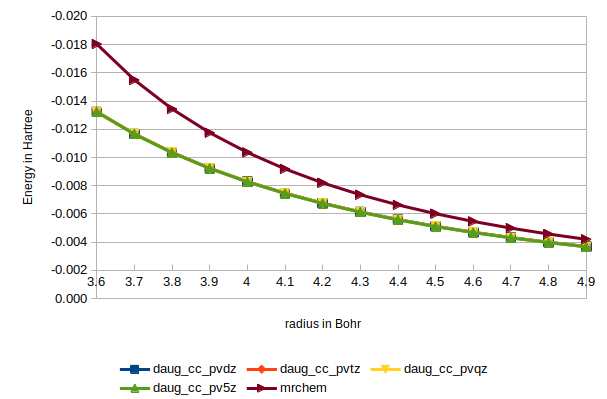
\includegraphics[width=0.75\linewidth]{img/Erdaugwat.png}
  \caption[Reaction field energy of \ce{H_2O}]{Reaction field energy of \ce{H_2O} in a water solution, calculated with relative precision $e-05$ in \mrchem and with double augmented basis sets in Gaussian}
  \label{fig:watEnergyplotsdaug}
\end{figure}

\begin{figure}[!htb]
  \centering
    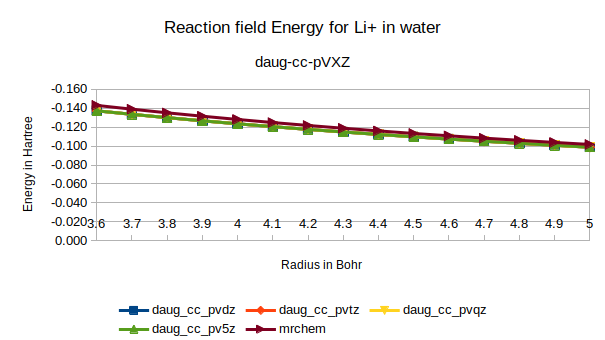
\includegraphics[width=0.75\linewidth]{img/Erdauglip.png}
  \caption[Reaction field energy of \ce{Li^+}]{Reaction field energy of \ce{Li^+} in a water solution, calculated with relative precision $e-05$ in \mrchem  and with double augmented basis sets in Gaussian}
  \label{fig:lipEnergyplotsdaug}
\end{figure}



\begin{figure}[!htb]
  \centering
    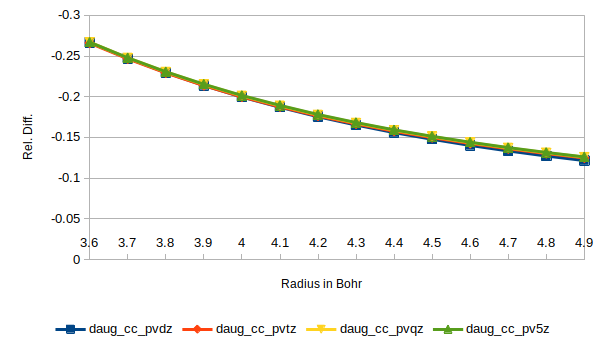
\includegraphics[width=\linewidth]{img/watdaugreldiff.png}
  \caption[Relative difference of \ce{H_2O} against Gaussian double augmented results]{Relative difference between the reaction field energy of \ce{H_2O} in a water solution calculated with with relative precision $e-05$ in \mrchem
   against double augmented basis sets in Gaussian}
  \label{fig:watreldiffdaug}
\end{figure}

\begin{figure}[!htb]
  \centering
  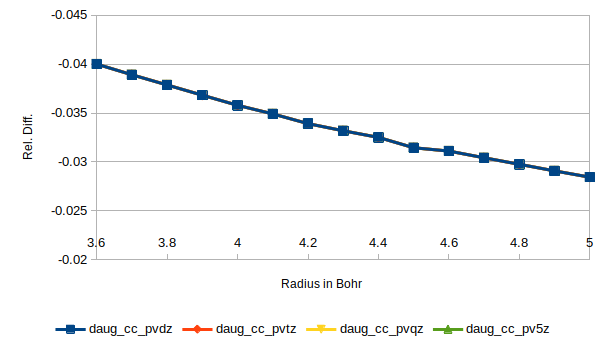
\includegraphics[width=\linewidth]{img/lipdaugreldiff.png}
  \caption[Relative difference of \ce{Li^+} against Gaussian double augmented results]{Relative difference between the reaction field energy of \ce{Li^+} in a water solution calculated with relative precision $e-05$ in \mrchem
  and with double augmented basis sets in Gaussian}
  \label{fig:lipreldiffdaug}
\end{figure}



\begin{figure}[!htb]
  \centering
    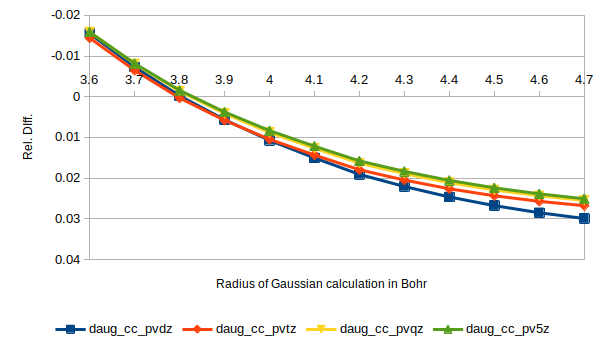
\includegraphics[width=\linewidth]{img/watdaugreldiff02.png}
  \caption[Relative difference of shifted radius \ce{H_2O} against Gaussian double augmented results]{Relative difference between the reaction field energy of \ce{H_2O} in a water solution calculated with with relative precision $e-05$ in \mrchem and radius $+ 0.2$ Bohr
  and with double augmented basis sets in Gaussian}
  \label{fig:watreldiff02daug}
\end{figure}

\begin{figure}[!htb]
  \centering
    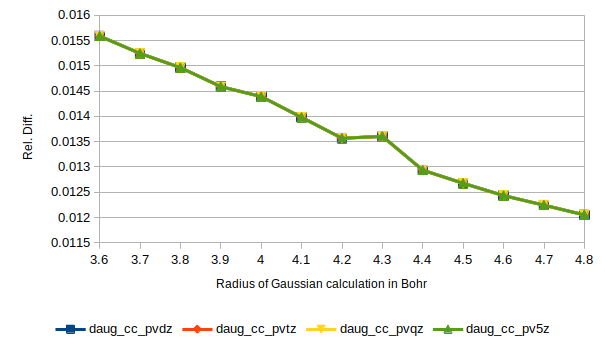
\includegraphics[width=\linewidth]{img/lipdaugreldiff02.png}
  \caption[Relative difference of shifted radius \ce{Li^+} against Gaussian double augmented results]{Relative difference between the reaction field energy of \ce{Li^+} in a water solution calculated with relative precision $e-05$ in \mrchem and radius $+ 0.2$ Bohr
  and with double augmented basis sets in Gaussian}
  \label{fig:lipreldiff02daug}
\end{figure}



\begin{figure}[!htb]
  \centering
  \begin{subfigure}[b]{0.75\linewidth}
    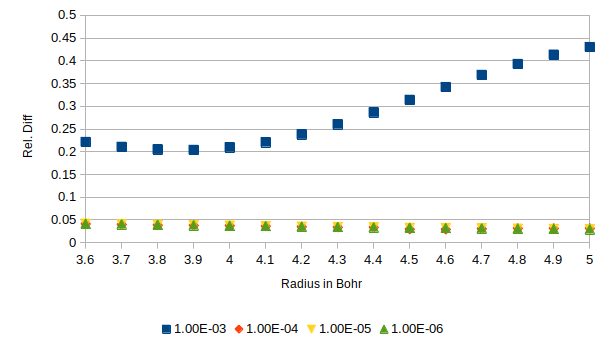
\includegraphics[width=\linewidth]{img/lipprecallreldiff.png}
    \caption{All precision values plotted}
  \end{subfigure}
  \begin{subfigure}[b]{0.75\linewidth}
    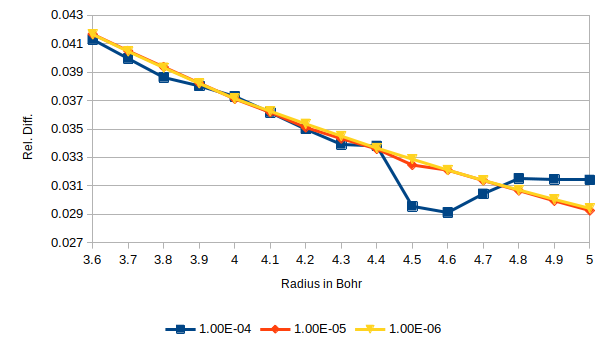
\includegraphics[width=\linewidth]{img/lipprecallreldiffexcl.png}
    \caption{All precision values plotted, except for precision value $1e-03$}
  \end{subfigure}
  \caption[Relative difference of \ce{Li^+} with different precision values against Gaussian results]{Relative difference between the reaction field energy of \ce{Li^+} in a water solution calculated with different relative precisions in \mrchem  and same calculations in Gaussian with daug-cc-pV5Z}
  \label{fig:lipprecreldef}
\end{figure}
\clearpage

\subsection{Comparison Tests}
The substrates studied in these tests are the same 4 substrates studied by Chipman in \cite{Chipman2002},
namely, \ce{H_2O}, \ce{NO^+}, \ce{CN^-} and \ce{CH_3CONH_2}. Two sets of comparison tests
were performed. Firstly, spherical cavity calculations where for each calculation the radius of the
cavity was varied. Secondly, molecular-shaped cavities calculations were performed on
all the substrates. Of the second type of test only two sets of radii were calculated, for
each substrate, cavities based on the Bondi radii multiplied by $1.2$, and the same cavities
but their radii were increased by $0.2$ Bohr. This is done to compensate for the
thickness of the cavity surface.


The results for the spherical cavity tests for \ce{H_2O} can be seen in Figures
\ref{fig:watEnergyplotsdaug} and \ref{fig:watreldiffdaug}, and the results for the
molecular-shaped tests for \ce{H_2O} can be seen on Table \ref{tab:watabcreldiff}.
For \ce{NO^+} the plots for the single sphere cavity tests can be seen in Figures
\ref{fig:nopEnergyplotsdaug} and \ref{fig:nopreldiffdaug} and the molecular
shape cavity test result can be seen in Table \ref{tab:nopabcreldiff}.
For \ce{CN^+} one can see the plots for the single sphere cavity on Figures
\ref{fig:cyanEnergyplotsdaug} and \ref{fig:cyanreldiffdaug} while the
molecular-shaped results are on Table \ref{tab:cyanabcreldiff}. The molecular-shaped
test for the incremented radii did not converge for \ce{CN^-}, but comparisons between
the standard scaled Bondi radii and the single sphere cavity can still be done.

Some of the data points for \ce{CN^-} and \ce{NO^+} are missing. The reason for this
is that the calculations for these values either never completed or gave extreme
outliers, due to yet not understood numerical instability. These outliers were removed from the plots
in order to better visualize the trend correctly converged values.
All of the available values, those which completed, can be seen in their corresponding
tables in Appendix \ref{Datatables}.

There are no single sphere cavity tests for \ce{CH_3CONH_2} due to the size of the molecule
making single sphere calculations extremely slow for both Gaussian and \mrchem.
The only tests that were ran where molecular-shaped tests. Gaussian did not converge
after 72 hours of running with \verb!daug-cc-pV5Z!, therefore, the comparison values
are missing from the tables. The \ce{CH_3CONH_2} results are presented in Table
\ref{tab:acetamidabcreldiff}.

The molecular-shaped cavity results shown are just the relative difference between
\mrchem and Gaussian values as shown in Equation \ref{eq:reldiff}. For the rest of the
tables see Appendix \ref{Datatables}.

\begin{figure}[!htb]
  \centering
    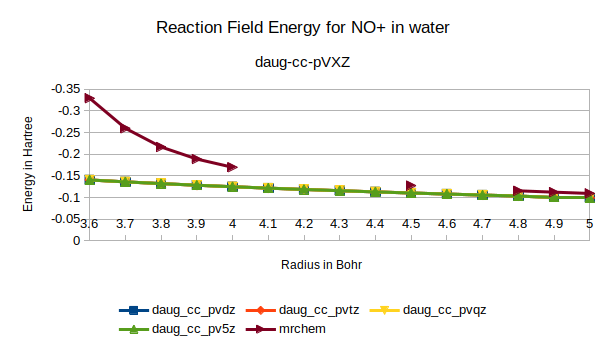
\includegraphics[width=\linewidth]{img/Erdaugnop.png}
  \caption[Energy plots for \ce{NO^+}]{Reaction field energy of \ce{NO^+} in a water solution, calculated with \mrchem
  and with different double augmented basis sets in Gaussian}
  \label{fig:nopEnergyplotsdaug}
\end{figure}

\begin{figure}[!htb]
  \centering
    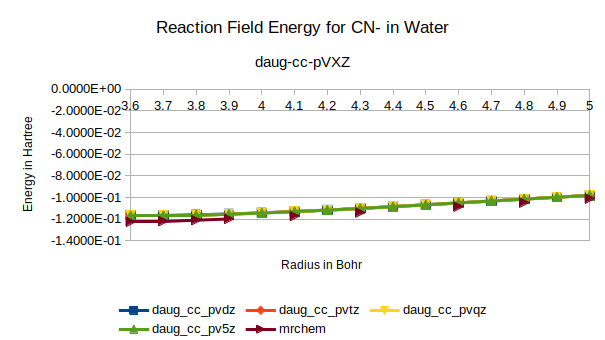
\includegraphics[width=\linewidth]{img/Erdaugcyan.png}
  \caption[Energy plots for \ce{CN^-}]{Reaction field energy of \ce{CN^-} in a water solution, calculated with \mrchem
  and with different basis sets in Gaussian}
  \label{fig:cyanEnergyplotsdaug}
\end{figure}

\begin{figure}[!htb]
  \centering
    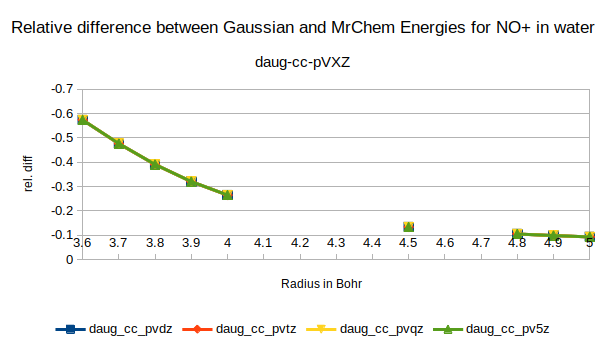
\includegraphics[width=\linewidth]{img/nopdaugreldiff.png}
    \caption[Relative difference between \ce{NO^+} and double augmented Gaussian results]{Relative difference between the reaction field energy of \ce{NO^+} in a water solution calculated with \mrchem
  and with different double augmented basis sets in Gaussian}
  \label{fig:nopreldiffdaug}
\end{figure}

\begin{figure}[!htb]
  \centering
    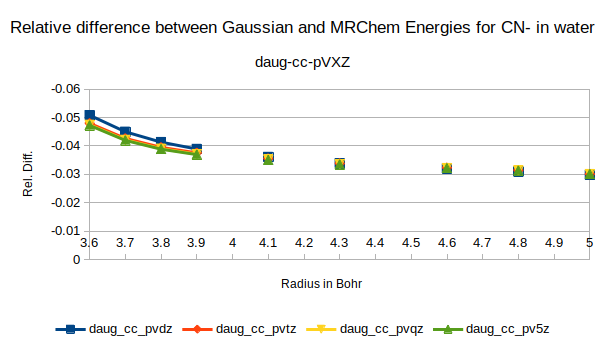
\includegraphics[width=\linewidth]{img/cyandaugreldiff.png}
  \caption[Relative difference between \ce{CN^-} and double augmented Gaussian results]{Relative difference between the reaction field energy of \ce{CN^-} in a water solution calculated with \mrchem
  and with different double augmented basis sets in Gaussian}
  \label{fig:cyanreldiffdaug}
\end{figure}


\begin{table}[htbp]
\caption[Relative difference between Gaussian and \mrchem results for \ce{H_2O}]{Relative difference between Gaussian and \mrchem results from molecular-shaped cavity  tests for \ce{H_2O}}
\begin{tabular}{l|r|r}
Basis & \multicolumn{1}{l|}{Van der Waals radii} & \multicolumn{1}{l|}{Van der Waals radii $+ 0.2$ Bohr} \\ \hline
cc-pVDZ & -0.150906543613473 & 0.04037455582641 \\
cc-pVTZ & -0.128295351717092 & 0.068079525814065 \\
cc-pVQZ & -0.128952645914318 & 0.067274158450387 \\
cc-pV5Z & -0.129254059406514 & 0.06690484347604 \\
aug-cc-pVDZ & -0.129130316675487 & 0.067056462579757 \\
aug-cc-pVTZ & -0.13428775618655 & 0.060737171340182 \\
aug-cc-pVQZ & -0.136838481699814 & 0.057611826417386 \\
aug-cc-pV5Z & -0.136314953280292 & 0.058253293670285 \\
daug-cc-pVDZ & -0.128163492341192 & 0.068241090054846 \\
daug-cc-pVTZ & -0.133787441562786 & 0.061350195266532 \\
daug-cc-pVQZ & -0.136489745183211 & 0.058039125198024 \\
daug-cc-pV5Z & -0.136235086647359 & 0.058351152406726 \\
\end{tabular}
\label{tab:watabcreldiff}
\end{table}


\begin{table}[htbp]
\caption[Relative difference between Gaussian and \mrchem results for \ce{NO^+}]{Relative difference between Gaussian and \mrchem results from molecular-shaped cavity  test for \ce{NO^+}}
\begin{tabular}{l|r|r}
Basis & \multicolumn{1}{l|}{Van der Waals radii} & \multicolumn{1}{l|}{Van der Waals radii $+ 0.2$ Bohr} \\ \hline
cc-pVDZ & -0.03598423 & 0.02044325 \\
cc-pVTZ & -0.03692221 & 0.01945037 \\
cc-pVQZ & -0.03747002 & 0.01887050 \\
cc-pV5Z & -0.03810456 & 0.01819881 \\
aug-cc-pVDZ & -0.03906862 & 0.01717832 \\
aug-cc-pVTZ & -0.03801963 & 0.01828871 \\
aug-cc-pVQZ & -0.03792710 & 0.01838665 \\
aug-cc-pV5Z & -0.03814585 & 0.01815510 \\
daug-cc-pVDZ & -0.03897379 & 0.01727870 \\
daug-cc-pVTZ & -0.03811073 & 0.01819228 \\
daug-cc-pVQZ & -0.03799786 & 0.01831176 \\
daug-cc-pV5Z & -0.03813936 & 0.01816197 \\
\end{tabular}
\label{tab:nopabcreldiff}
\end{table}


\begin{table}[!htbp]
\caption[Relative difference between Gaussian and \mrchem results for \ce{CN^-}]{Relative difference between Gaussian and \mrchem results from molecular-shaped cavity  test for \ce{CN^-}}
\begin{tabular}{l|r}
Basis & \multicolumn{1}{l|}{Van der Waals radii} \\ \hline
cc-pVDZ & 0.01805797 \\
cc-pVTZ & 0.00402722 \\
cc-pVQZ & -0.00689520 \\
cc-pV5Z & -0.01760704 \\
aug-cc-pVDZ & -0.02534307 \\
aug-cc-pVTZ & -0.02484616 \\
aug-cc-pVQZ & -0.02473155 \\
aug-cc-pV5Z & -0.02453156 \\
daug-cc-pVDZ & -0.02428967 \\
daug-cc-pVTZ & -0.02475331 \\
daug-cc-pVQZ & -0.02472359 \\
daug-cc-pV5Z & -0.02449823 \\
\end{tabular}
\label{tab:cyanabcreldiff}
\end{table}

\begin{table}[htbp]
\caption[Relative difference between Gaussian and \mrchem results for \ce{CH_3CONH_2}]{Relative difference between Gaussian and \mrchem results from molecular-shaped cavity  test for \ce{CH_3CONH_2}}
\begin{tabular}{l|r|r}
Basis & \multicolumn{1}{l|}{Van der Waals radii} & \multicolumn{1}{l|}{Van der Waals radii$+0.2$ Bohr} \\ \hline
cc-pVDZ & -0.186177328600554 & -0.025757341450533 \\
cc-pVTZ & -0.13954657945224 & 0.030065218693051 \\
cc-pVQZ & -0.12431319516031 & 0.048301393885559 \\
cc-pV5Z & -0.12131273376434 & 0.051893303511593 \\
aug-cc-pVDZ & -0.113966441504817 & 0.060687690240943 \\
aug-cc-pVTZ & -0.120388767462925 & 0.052999401212647 \\
aug-cc-pVQZ & -0.122585402181545 & 0.050369767849829 \\
aug-cc-pV5Z & -0.122435027608944 & 0.050549784121847 \\
daug-cc-pVDZ & -0.117198265984418 & 0.056818811449993 \\
daug-cc-pVTZ & -0.121288328616877 & 0.051922519379598 \\
daug-cc-pVQZ & -0.122478065257119 & 0.050498262931483 \\
\end{tabular}
\label{tab:acetamidabcreldiff}
\end{table}
\clearpage


\subsection{Variational implementation tests}
Figures \ref{fig:watvarEr} and \ref{fig:lipvarEr} show the reaction field energy
calculated with the variational implementation for \ce{H_2O} and \ce{Li^+},
respectively. Figures \ref{fig:watreldiffvardaug} and \ref{fig:lipreldiffvardaug} show the
relative difference as calculated with Equation \ref{eq:reldiff} for \ce{H_2O} and \ce{Li^+},
respectively.

\begin{figure}[!htb]
  \centering
  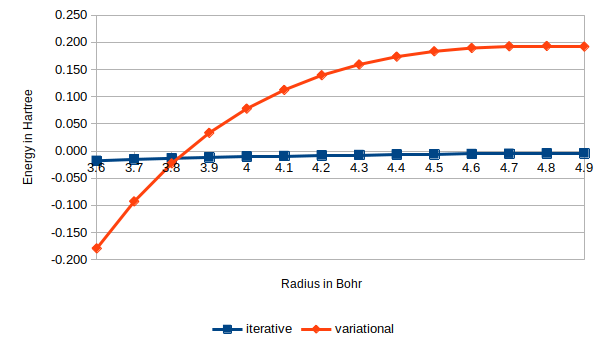
\includegraphics[width=0.75\linewidth]{img/watvarEr.png}
  \caption{Reaction field energy for \ce{H_2O} in water using the variational and iterative implementation}
  \label{fig:watvarEr}
\end{figure}

\begin{figure}[!htb]
  \centering
  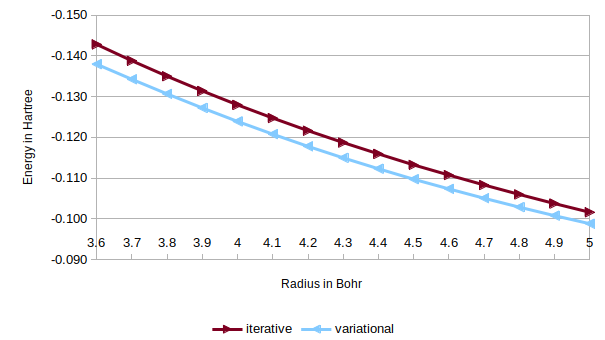
\includegraphics[width=0.75\linewidth]{img/lipvarEr.png}
  \caption{Reaction field energy for \ce{Li^+} in water using the variational and iterative implementation}
  \label{fig:lipvarEr}
\end{figure}

\begin{figure}[!htb]
  \centering
    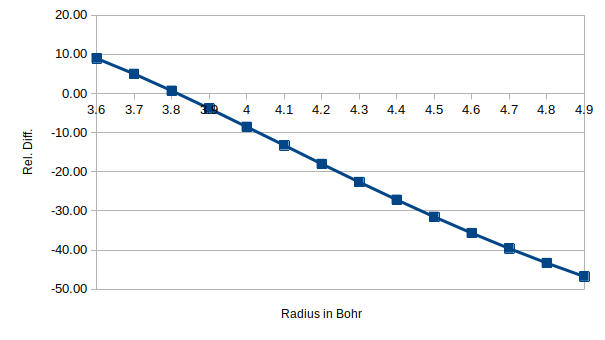
\includegraphics[width=\linewidth]{img/watitervarreldiff.png}
  \caption{Relative difference between the reaction field energy of \ce{H_2O} calculated with the variational implementation against the iterative implementation}
  \label{fig:watreldiffvardaug}
\end{figure}

\begin{figure}[!htb]
  \centering
    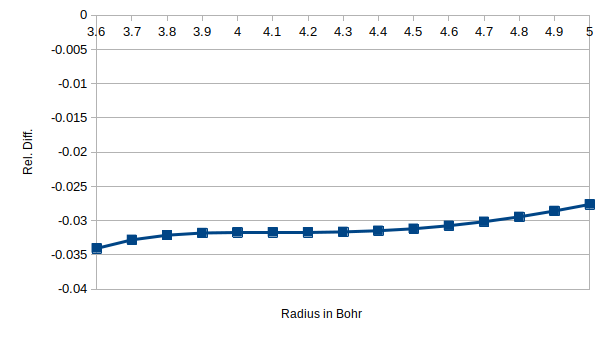
\includegraphics[width=\linewidth]{img/lipitervarreldiff.png}
  \caption{Relative difference between the reaction field energy of \ce{H_2O} calculated with the variational implementation against the iterative implementation}
  \label{fig:lipreldiffvardaug}
\end{figure}
\clearpage


\section{Discussion}
\subsection{Theoretical correctness }
The results for the integral of the surface charge distribution $\gamma_s$ for
both dielectric constants of 2 and 80 are on Tables \ref{tab:Intgamma2} and \ref{tab:intgamma80}
respectively. These results must coincide with  exact value calculated with Equation \ref{eq:Reactioncharge}
if the implementation is theoretically correct. We can see that, since the relative difference is
so small, that the implementation is correct for both big and small dielectric constants.
The values for $\epsinf = 80$ have a bit larger relative difference in comparison, which stems from
the fact that the implementation has hardships in solving solvation systems with big dielectric constants.
Increasing the precision of the calculations decreases the relative difference, as expected.

Increasing the radius does not improve the differences of the integrals, except for
$\epsinf = 2 \text{ with } \sigma = 0.1 \text{ and } prec. = 1e-4$, and for
$\epsinf = 80 \text{ with } \sigma = 0.2 \text{ and } prec. = 1e-4$ where it improves by
$0.1\% \text{ for } \epsinf = 2$ and $0.03\%$ for $\epsinf = 80$. The cause for
this decrease in the quality of the \mrchem results might be because of the surface
charge effect being diminished by the bigger cavity. The reason it gets better at
only two sets of parameters might be caused by numerical noise, given the size of
the variation.
The same  behavior is seen for tighter surfaces. The difference worsens
when increasing tightness, and where it gets better is most likely because of numerical noise,
given the size of the variation. These two observation show the difficulty this implementation still
has at working with sharp transitions and larger surface areas.

The energies, on the other hand, do not have the constraint of needing to be exactly the same as
the Born model values. This is simply because the Born model is a model in which
the cavity surface is a sharp transition. We can see that this is the case since the
relative difference increases or decreases by very small  values when increasing the
relative precision of the calculations, telling us that
the variation of our values between themselves is much smaller than  the difference
with the Born model.
It was expected as well, that when the width of our cavity surface becomes small
compared to the radius our results would resemble
the Born results more. Two ways of decreasing the width of the surface relative to the
size of the cavity exist, either by increasing the  radius and/or by decreasing the width of the transition.
Both of these relations hold true, in our results, for both dielectric constants.


The relative differences for the $\epsinf = 80$ are not as good as for $\epsinf = 2$.
The most likely cause is the transition becomes steeper relative
to the width and radius parameters due to the high difference between $\epsinf \text{ and } \epso$.
This leads to \mrchem having difficulties projecting the cavity, which in turn,
increase the numerical noise in the calculation.

\subsection{Parametrization }
The values for \ce{H_2O} reaction energy with a cavity radius of $5$ Bohr diverged, therefore
we removed them in order to better visualize the trends.
We can see in Figures \ref{fig:watreldiffdaug} and \ref{fig:lipreldiffdaug}
that the relative difference decays, diminishes to a stable value, the bigger the cavity is. The method Gaussian
uses to calculate the reaction field describes the transition from inside the
cavity to the outside as happening at a boundary, this being the surface of the cavity.
The problem is solved at the surface of the cavity, which is assumed to be two dimensional,
so the transition is noncontinuous, as explained in Chapter \ref{chap:Solvent_effect}.
Our cavity is defined as an analytical transition with a parameter $\sigma$ which
controls the width of the cavity surface, so that we get a smooth transition
between the inside and the outside of the cavity.

Two main factors are responsible for the decay in relative difference that we observe.
Firstly, the bigger the radius, the smaller the difference is relative to the
size of the cavity. This means that at larger distances our cavity resembles
more and more that of a discontinuous transition such as the ones used by
Gaussian. The second factor is the amount of the charge density that is contained within
the cavity. The effect of this can be seen on the tests that followed.

As we can see on the Figures \ref{fig:watreldiff02daug} and \ref{fig:lipreldiff02daug}
there is a significant improvement on the relative difference when we compare with
bigger radii of \mrchem calculations to smaller radii of Gaussian calculations.
This is caused by the smooth cavity. Since the transition is wider in our implementation
there is more density that is situated outside the cavity than in cavities of same radius
from Gaussian calculations. This was accounted for when we increased the radii, and we still
see the same decay in difference that we saw in the standard comparison.

The graphs from Figure \ref{fig:lipprecreldef} tell us two things about our results:
Firstly at precision lower than $1e-03$ we get results that are at least $20\%$ different
than the best Gaussian results we could run for small radii and diverge from the
Gaussian results for bigger radii. Secondly we see that we don't need a relatively
high precision to get stable results which are consistent with greater previsions and
that also approach the Gaussian results at bigger radii.

On the other hand, it is hard to decide if this is applicable to bigger systems,
as the Lithium cation is fairly simple, whereas
other systems might not be so simple.

\subsection{Comparison }
Same as with the tests for \ce{Li^+} and \ce{H_2O}, the Figures \ref{fig:nopreldiffdaug}
and  \ref{fig:cyanreldiffdaug} show that both relative differences for \ce{CN^-}
and \ce{NO^+} decay at higher radii.

The relative differences for the results for \ce{NO^+}  seem to decay faster
than the other molecules, but it
is hard to see due to the lack of data points. Assuming that it decays faster,
one can explain this as being due to the fact that the electron density is
closer to the atoms, making it easier for the cavity to contain most of it.
The opposite can be seen for \ce{CN^-}. The explanation for this might go through
the same line of thought as that for \ce{NO^+}, but now since the molecule is negatively
charged, the density is more diffuse, making it harder to contain it in its entirety.

The divergence around the interval $(4.0, 4.7)$ can be attributed to the way the
functions are projected. The cavity function is very sharp at the transition. In order to
project it correctly one needs to go to very low scales.
Additionally, the intervals are
powers of two, meaning that there is always the discontinuity from the wavelets at the
$4.0$ point, which is hard to correct. This discontinuity brings forth numerical
noise that gets amplified when the derivative of the function is calculated to solve the
\ac{GPE}.
These errors occur in this implementation as it is still in development. These
problems are expected to be diminished or removed in future revisions. One way we
could attempt to fix is by defining a better derivative for the cavity.
Fosso--Tande defined the derivative of the cavity as combinations of analytical
derivatives \cite{FossoTande:2013ka}. This definition supposedly would help
remove numerical noise at the transition, since one can create these analytical
derivatives before projecting them into the \ac{MW} basis.

The tables for the molecular-shaped cavity tests  show us that for most the molecules, the
relative difference doesn't vary too much when going to molecular-shaped cavity or that it gets
much better, as is the case for \ce{NO^+} in Table \ref{tab:nopabcreldiff}.
It can be seen that, while its spherical cavity plot, Figure \ref{fig:nopreldiffdaug}, does not go
lower than a relative difference of $10\%$, its molecular-shaped cavity tests have a relative difference
of less than $4\%$. The same can be said for the results for \ce{CN^-}, in Table \ref{tab:cyanabcreldiff},
which got to less than $3\%$ from the Gaussian results, while it never approached $10\%$
with spherical cavity, Figure \ref{fig:cyanreldiffdaug}.

The \ce{H_2O} results, in Table \ref{tab:watabcreldiff} do not go too far from the best relative difference
shown in Figure \ref{fig:watreldiffdaug}. They do significantly better when increasing
the radius of the interlocking spheres, a decrease in the relative difference of
around $6-9\%$. This decrease is seen in the other molecules as well, where,
for \ce{NO^+}, the decrease is around $1-2\%$.

\ce{CH_3CONH_2}, in Table \ref{tab:acetamidabcreldiff} has a difference of at
best $11.4\%$ and at worst $18.6\%$. Increasing the radii of the interlocking spheres
has the same effect that was observed for \ce{H_2O}, but stronger. Here they decrease by
$ 5-16\%$.  This tells us that in \mrchem, in order to get comparable results to
Gaussian, one need to define a cavity that is a bit bigger than the one used in Gaussian.
This makes sense as the cavity surface, because of the width, starts earlier for us
than it does for Gaussian. This leads to more of the density escaping. Increasing the
radius gives us a cavity that is effectively the same as Gaussian's.

\subsection{Variational implementation}
The results for the variational implementation of the \ac{GPE} for \ce{H_2O} and \ce{Li^+}
is shown in Figures \ref{fig:watreldiffvardaug} and \ref{fig:lipreldiffvardaug}
respectively.

Ideally, the results from the iterative and variational implementation should be
almost equal, with differences between them being for the most part caused by numerical
noise. This is because we are using the same \ac{GPE}, but different implementation,
for both of them.

\ce{Li^+} behaves almost as expected, with very small differences between implementations,
which can be explained as numerical noise. \ce{H_2O} on the other hand shows signs that,
for bigger systems, the errors are not numerical noise only. The \ce{H_2O} differences imply
that there is an error in the implementation, which gets augmented for bigger systems.
This is further strengthened by the fact that the variational values for the other
molecules had the same trend, as can be seen in the Tables of Appendix \ref{Datatables}.

Something worth noting is that the values appear to behave systematically,
which strengthens the possibility of something being implemented wrongly, and most
importantly, that it can be accounted for and corrected in future revisions of
this implementation.

\section{Concluding remarks}
The theoretical correctness tests showed that the implementation is, at its base,
theoretically correct.

We saw that when increasing the radii of the cavity in calculations, the difference
between the Gaussian calculations and the \mrchem calculations decayed, as is
expected.
Having a tighter precision than $1e-4$ helps to have better results, but is not entirely
necessary, as the difference between the models is larger than the improvement upon
moving to better precision values.

We see that all the solutes used in \cite{Chipman2002} have relative differences that
decay with bigger radii. We also saw that using bigger \mrchem cavities where Gaussian
used smaller gave us better relative differences in molecular-shaped Cavities.
The \mrchem calculations did not converge for some values of \ce{CN^-} and \ce{NO^+}
which is most likely caused by instabilities in the derivatives of the cavity, which
can be improved by following Fosso--Tande \cite{FossoTande:2013ka}.

The variational implementation gives acceptable results for small systems such
as \ce{Li^+} but for bigger systems, it shows clear signs of errors in the implementation.
The variational implementation is still in its early days when it comes to development,
and the results still behave systematically, which tells us that they can be accounted for and
improved upon.
We have also seen that for most of our comparisons we could not expect out values to actually
converge to what we were testing against. This is because there still are not many
equivalent implementations to test against.

\section{Areas of improvement/future development}
Given that the iterative values gave results as expected we can say that the
implementation is correct. An improvement would be to try to change the cavity
definition so as to take into account more of the electron density. One way that is
possible right now is to decrease the width of the transition, another is to simply use
bigger cavities as these are shown to give better results. Both of those are possible
with the implementation used now, but decreasing the width of the transition might
make the cavity harder to project.

A better solution to this is to implement the derivative of the caivty as
a combination of analytical derivatives, as Fosso--Tande did in \cite{FossoTande:2013ka}, which
might let us get better results with the same parameters used in the tests of this chapter.

The goal in the future is to apply these solutions and test if they better the
results of the variational method. After that we will start seeing how molecular properties
are affected by this.

Another goal is to attempt better stability at sharper cavity surfaces as there
is clearly a trend where the narrower the surface, the harder it is to actually
converge it.


\begin{acronym}
\acro{AUS}[\href{https://www.sigma2.no/content/advanced-user-support}{AUS}]{Numerical Methods in Quantum Chemistry}
\acro{BO}{Born-Oppenheimer}
\acro{CTCC}[\href{http://www.ctcc.no}{CTCC}]{Centre for Theoretical and Computational Chemistry}
\acro{DC}{Dielectric Continuum}
\acro{DFT}{Density Functional Theory}
\acro{EFP}{Effective Fragment Potential}
\acro{EU}{European Union}
\acro{HF}{Hartree-Fock}
\acro{Hylleraas}[\href{https://www.mn.uio.no/hylleraas/english/}{Hylleraas}]{Hylleraas
  Centre for Quantum Molecular Sciences}
\acro{HPC}{High Performance Computing}
\acro{KTH}{Royal Institute of Technology}
\acro{LDA}{Local Density Approximation}
\acro{MCD}{Magnetic Circular Dichroism}
\acro{MCSCF}{Multiconfiguration Self Consistent Field}
\acro{MM}{Molecular Mechanics}
\acro{MW}{Multiwavelet}
\acro{NFR}{Norwegian Research Council}
\acro{NMQC}[\href{http://www.ctcc.no/events/conferences/2015/numeric-conference/}{NMQC}]{Numerical Methods in Quantum Chemistry}
\acro{NOTUR}[\href{https://www.notur.no/}{NOTUR}]{Norwegian Metacenter for Computational Science}
\acro{PCM}{Polarizable Continuum Model}
\acro{PI}{Primcipal Investigator}
\acro{QC}{Quantum Chemistry}
\acro{QM}{Quantum Mechanics}
\acro{QM/MM}{Quantum Mechanics/Molecular Mechanics}
\acro{ROA}{Raman Optical Activity}
\acro{SC}{semiconductor}
\acro{SCF}{Self Consistent Field}
\acro{SHG}{Second Harmonic Genertation}
\acro{STSM}{Short-term scientific mission}
\acro{TPA}{Two-Photon Absorption}
\acro{WP}{Work Package}
\acro{CBS}{Complete Basis Set}
\acro{TCG}{Theoretical Chemistry Group}
\acro{vdW}{van der Waals}
\acro{SE}{Schrödinger Equation}
\acro{PES}{Potential Energy Surface}
\acro{LCAO}{Linear Combination of Atomic Orbitals}
\acro{MRA}{Multi-Resolution Analysis}
\acro{NS}{Nonstandard}
\end{acronym}

\biblio
\end{document}
